\documentclass[11pt]{article}

% load some asm stuff -
\usepackage{amssymb}
\usepackage{amsmath}
\usepackage{amsthm}
%\usepackage{palatino,lettrine}
\usepackage{fancyhdr}
\usepackage{epsfig}
\usepackage[round,comma,sort]{natbib}
\usepackage{simplemargins}
\usepackage{setspace}

\usepackage[margin=0pt,font=small,labelfont=bf]{caption}

\bibliographystyle{plos2009}

% Set the size
%\textwidth = 6.75 in
%\textheight = 9.75 in
%\oddsidemargin = 0.0 in
%\evensidemargin = 0.0 in
%\topmargin = 0.01 in
%\headheight = 0.0 in
%\headsep = 0.25 in
%\parskip = 0.15in
\doublespace

\setallmargins{1in}

\newtheorem{example}{Example}[section]
\newtheorem{thm}{Theorem}[section]
\newtheorem{property}{Property}[section]

\theoremstyle{definition}
\newtheorem{defn}[thm]{Definition}

\makeatletter
\renewcommand\subsection{\@startsection
	{subsection}{2}{0mm}
	{-0.05in}
	{-0.5\baselineskip}
	{\normalfont\normalsize\bfseries}}
\renewcommand\subsubsection{\@startsection
	{subsubsection}{2}{0mm}
	{-0.05in}
	{-0.5\baselineskip}
	{\normalfont\normalsize\itshape}}
\renewcommand\paragraph{\@startsection
	{paragraph}{2}{0mm}
	{-0.05in}
	{-0.5\baselineskip}
	{\normalfont\normalsize\itshape}}
\makeatother
\linespread{1.2}

\fancypagestyle{proposal}{\fancyhf{}%
	\fancyhead[RO,LE]{\thepage}%
	\fancyhead[LO,RE]{CHEME 2880 Week 4: Metabolic Flux Analysis and Flux Balance Analysis}%
	\renewcommand\headrulewidth{1pt}}
\pagestyle{proposal}

% Single space'd bib -
\setlength\bibsep{0pt}

\renewcommand{\rmdefault}{phv}\renewcommand{\sfdefault}{phv}

% Change the number format in the ref list -
\renewcommand{\bibnumfmt}[1]{#1.}

% Change Figure to Fig.
\renewcommand{\figurename}{Fig.}

%Joycelyn Chan, Joshua Lequieu, Michael Paull, Chidanand Balaji, Ryan Tasseff
%Our derivation follows closely the earlier development of Fredrickson \citep{Fredrickson:1976fk}.


% Begin ...
\begin{document}
\setcounter{page}{1}




\section{How can we solve the intracellular material balance equations?}
We can solve intracellular material balance equations numerically using common software packages such as MATLAB,
if we knew the functional form of the fluxes and values for the kinetic parameters which appear in the fluxes.
However, the functional form of the fluxes or their associated parameter values are often difficult (sometimes impossible) to estimate.
Two alternative strategies, metabolic flux analysis (MFA) and flux balance analysis (FBA), have been used to estimate the intracellular fluxes at or near an intracellular
steady-state.

\subsection*{Metabolic Flux Analysis (MFA).}
Metabolic flux analysis relies upon a pseudo steady-state assumption to reduce the intracellular material balance equations to algebraic equations given in matrix-vector form by:
\begin{equation}\label{eqn-mfa-ss-w-metabolites}
	\mathbf{S}\mathbf{v} + \mathbf{T}\mathbf{q} -\mu\mathbf{I}\mathbf{x}^{*}\simeq\mathbf{0}
\end{equation}where $\mathbf{x}^{*}$ denotes the species abundance vector at steady-state.
The quantity $\mathbf{S}$ denotes the stoichiometric matrix ($\mathcal{M}\times{\mathcal{R}}$),
$\mathbf{T}$ denotes the transport (or exchange) matrix ($\mathcal{M}\times{\mathcal{T}}$) and the $\mathbf{I}$ denotes the ($\mathcal{M}\times{\mathcal{M}}$) identity matrix.
Eqn \eqref{eqn-mfa-ss-w-metabolites} has two sets of unknowns, the states and the fluxes. Without experimental measurements, we have no means to estimate $\mathbf{x}^{*}$.
Moreover, we know the dilution due to growth terms ($\mu\mathbf{I}\mathbf{x}^{*}$) are small.
Thus, we typically drop these dilution terms to arrive at:
\begin{equation}\label{eqn-mfa-ss-wno-metabolites}
	\mathbf{S}\mathbf{v} + \mathbf{T}\mathbf{q} \simeq\mathbf{0}
\end{equation}Eqn \eqref{eqn-mfa-ss-wno-metabolites} are $\mathcal{M}$ algebraic equations in the unknown intracellular fluxes $v_{1},\hdots,v_{\mathcal{R}}$ and transport fluxes
$q_{1},\hdots,q_{\mathcal{T}}$. Typically, $\mathcal{M}<\mathcal{R}+\mathcal{T}$ which means that no unique flux solution can be found.
However, we can potentially measure some of the transport fluxes that carry material into and from the cells. Denote the subset of \emph{measured} fluxes
as $\vartheta_{m}$ ($\mathcal{E}\times{1}$ column vector), and all other fluxes as $\vartheta_{u}$ ($\mathcal{U}\times{1}$ column vector).
We can then redefine the stoichiometric balances as:
\begin{equation}\label{eqn-mfa-ss-wno-metabolites-split}
	\mathbf{\Sigma}\vartheta_{u} + \mathbf{\Phi}\vartheta_{m} \simeq\mathbf{0}
\end{equation}where $\mathbf{\Phi}$ contains the columns corresponding to the measured fluxes ($\mathcal{M}\times\mathcal{E}$), while the $\mathbf{\Sigma}$ matrix contains
the columns corresponding to \emph{unmeasured} fluxes ($\mathcal{M}\times\mathcal{U}$).
Eqn \eqref{eqn-mfa-ss-wno-metabolites-split} can be solved for the \emph{unmeasured} fluxes $\vartheta_{u}$:
\begin{equation}
	\vartheta_{u}\simeq-\mathbf{\Sigma}^{\#}\mathbf{\Phi}\vartheta_{m}
\end{equation}where $\mathbf{\Sigma}^{\#}$ is a $\mathcal{U}\times\mathcal{M}$ \emph{generalized} matrix inverse.

\subsubsection*{What is $\mathbf{\Sigma}^{\#}$ and when does it exist?}
The matrix $\mathbf{\Sigma}^{\#}$ is the generalized inverse of the stoichiometric matrix corresponding to the \emph{unmeasured} fluxes. The form of $\mathbf{\Sigma}^{\#}$ depends
upon the shape and the \emph{rank} of $\mathbf{\Sigma}$.
The definition of the $\mathbf{\Sigma}$ and $\mathbf{\Phi}$ arrays influences our ability to solve the intracellular material balances. The structure of these arrays
is controlled practically by which fluxes are measured. Measurement selection is influenced by several factors, technical concerns regarding the measurement
technology, the cost of measurements as well as the time required to make measurements.

\begin{itemize}

\item{$\mathcal{M}>\mathcal{U}$: \textbf{Overdetermined System of Equations.}
Overdetermined systems are characterized by more equations than unknowns and have no single \emph{regular} solution, in other
words, no single solution will simultaneously satisfy all the equations. The problem of determining the solution to an overdetermined
system can be recast as a least-squares problem of the form:
\begin{equation}\label{eq-ose}
\min_{\mathbf{\vartheta_{u}}}\bigl(\mathbf{\Sigma\vartheta_{u}}-\mathbf{b}\bigr)^{T}\bigl(\mathbf{\Sigma\vartheta_{u}}-\mathbf{b}\bigr)
\end{equation}where
\begin{equation}
\mathbf{b}\equiv-\mathbf{\Phi\vartheta_{m}}\left(t\right)
\end{equation}
Equation \eqref{eq-ose} can be analytically solved by standard calculus to yield the solution:
\begin{equation}\label{eq-right}
\mathbf{\vartheta_{u}}=\left(\mathbf{\Sigma^{T}\Sigma}\right)^{-1}\mathbf{\Sigma^{T}b}
\end{equation}In this case the quantity $\mathbf{\Sigma}^{\#}$ is given by:
\begin{equation}
\mathbf{\Sigma}^{\#} = \mathbf{\Sigma^{L}}\equiv\left(\mathbf{\Sigma^{T}\Sigma}\right)^{-1}\mathbf{\Sigma^{T}}
\end{equation}denotes a \emph{left} inverse (sometimes called the Moore-Penrose inverse, generalized inverse or pseudo inverse).
For the least-squares solution Equation
\eqref{eq-right} to exist, the condition
\begin{equation}
\det\mathbf{\Sigma^{T}\Sigma}\neq{0}
\end{equation}must be satisfied.}

\item{$\mathcal{M}<\mathcal{U}$: \textbf{Underdetermined System of Equations.}
Underdetermined systems are characterized by an $\infty$-solutions as $n$ unknowns can be written in terms of the remaining $m-n$
unknowns which in the general case take on arbitrary values. The solution of an underdetermined system of LAEs can be posed
as a constrained least-squares minimization problem of the form:
\begin{equation}\label{eq-under}
\min_{\mathbf{u}}\frac{1}{2}\mathbf{\vartheta_{u}}^{T}\mathbf{\vartheta_{u}}
\end{equation}subject to:
\begin{equation}
\mathbf{\Sigma\vartheta_{u}}=\mathbf{b}
\end{equation}where
\begin{equation}
\mathbf{b}\equiv-\mathbf{\Phi\vartheta_{m}}\left(t\right)
\end{equation}
Problem \eqref{eq-under} has been solved analytically using standard techniques from calculus to yield the solution:
\begin{equation}
\mathbf{\vartheta_{u}}=\mathbf{\Sigma}^{T}\left(\mathbf{\Sigma\Sigma}^{T}\right)^{-1}\mathbf{b}
\end{equation}
The quantity
\begin{equation}\label{eq-left}
\mathbf{\Sigma}^{\#} = \mathbf{\Sigma^{R}}\equiv\mathbf{\Sigma^{T}}\left(\mathbf{\Sigma\Sigma^{T}}\right)^{-1}
\end{equation}denotes a \emph{right} inverse.
For the least-squares solution Equation
\eqref{eq-left} to exist, the condition
\begin{equation}
\det\mathbf{\Sigma\Sigma^{T}}\neq{0}
\end{equation}must be satisfied.}

\item{$\mathcal{M}=\mathcal{U}$: \textbf{Square Systems.}
When the number of equations equals the number of unknowns the system is said to be \emph{square}. Square systems can be
solved by several different techniques, including directly determining the matrix inverse $\mathbf{S}^{-1}$, i.e.,
\begin{equation}\label{eq-square-soln}
\mathbf{\vartheta_{u}}=-\mathbf{\Sigma}^{-1}\mathbf{\Phi\vartheta_{m}}\left(t\right)
\end{equation}Solution \eqref{eq-square-soln} exists as along as:
\begin{equation}
\det\left(\mathbf{\Sigma}\right)\neq{0}
\end{equation} The direct computation of the inverse for square systems is \emph{very} computationally expensive, so in practice
other techniques, such as Gauss Elimination, Gauss Jordan Elimination or iterative techniques are used to calculate the flux
vector $\mathbf{\vartheta_{u}}$.
}
\end{itemize}

An alternative to computing the determinant to check the existence of the matrix inverse, is to compute the rank. The rank of the $N\times{M}$ matrix $\mathbf{A}$ given by:
\begin{equation}
	rank\left(\mathbf{A}\right)\leq\min\left(N,M\right)
\end{equation}is a measure of the independent information contained in the rows and columns of a matrix. Arrays with linearly independent rows and columns have full rank, while arrays with linearly dependent components are not full rank. For a determinant to be non-zero, an array has to be full rank. Performing a rank test is more efficient that computing the determinant of a matrix, especially for non-square matrices.

\begin{figure*}[h!]\centering
\psfig{file=figs/Simple-network-example.eps,width=0.8\textwidth}
\caption{Schematic of simple metabolic reaction network. This system has a total of six metabolites and seven reactions. The intracellular metabolites (metabolites $A,B$ and $C$) are often treated as balanced (no accumulation) while the extracellular metabolites ($A_{x},B_{x}$ and $C_{x}$) are not conserved (can accumulate). The blue-oval denotes the cell boundaries, where $q_{j}$ denotes flux across these boundaries ([mmol/gdw-hr]) and $v_{k}$ denotes the intracellular fluxes.}\label{fig-system}
\end{figure*}

\begin{example}
	Estimate the intracellular fluxes for the simple reaction network shown in Fig. \eqref{fig-system} using metabolic flux analysis (MFA).
	Assuming we measured all three transport fluxes, the stoichiometric and transport arrays for this network are given by:
	\begin{equation}
	\mathbf{\Sigma} =
	\begin{bmatrix}
		-1 & -1 & 0 & 1 \\
		1 & 0 & 1 & -1 \\
		0 & 1 & -1 & 0 \\
	\end{bmatrix}
	\end{equation} and
	\begin{equation}
		\mathbf{\Phi} =
		\begin{bmatrix}
			1 & 0 & 0 \\
			0 & -1 & 0 \\
			0 & 0 & -1 \\
		\end{bmatrix}
	\end{equation}
	The stoichiometric matrix $\mathbf{\Sigma}$ is not square nor does it have full rank $rank\left(\mathbf{\Sigma}\right)$ = 2.
	Thus, even the pseudo inverse is not defined for this set of measured fluxes, suggesting we need to change our experimental design.
	If we measure only $q_{1}$ and $q_{2}$, the stoichiometric and transport arrays become:
	\begin{equation}
	\mathbf{\Sigma} =
	\begin{bmatrix}
		-1 & -1 & 0 & 1 & 0 \\
		1 & 0 & 1 & -1 & 0 \\
		0 & 1 & -1 & 0 & -1 \\
	\end{bmatrix}
	\end{equation} and
	\begin{equation}
		\mathbf{\Phi} =
		\begin{bmatrix}
			1 & 0 \\
			0 & -1 \\
			0 & 0 \\
		\end{bmatrix}
	\end{equation}which has full rank $rank\left(\mathbf{\Sigma}\right)$ = 3.
	We can compute a right inverse and solve for $\vartheta_{u} = \left(v_{1},v_{2},v_{3},q_{3}\right)$.
	If we assume $q_{1} = 1.0$ and $q_{2} = 0.5$, the flux solution is shown in Fig. \eqref{fig-bad-flux-solution}.

	\begin{figure*}[h!]\centering
	\psfig{file=figs/Simple-network-example-flux-solution.eps,width=0.4\textwidth}
	\caption{Example flux solution for $q_{1} = 1.0$ and $q_{2} = 0.5$. While the overall material balance is consistent, some estimated intracellular fluxes ($v_{3}$ and $v_{4}$) violate non-negativity. }\label{fig-bad-flux-solution}
	\end{figure*}
	We can resolve the non-negativity issue by further constraining the relationships between the fluxes.
	However, the formulation of these additional constraints are case specific.

\end{example}

\subsection*{Flux balance analysis (FBA).}
Flux balance analysis (FBA) is another strategy to estimate intracellular fluxes.
FBA was developed by Palsson and coworkers to estimate fluxes of genome scale models of \emph{E. coli} \citep{Edwards:2000yq}.
The FBA problem recasts the estimation of intracellular fluxes as a Linear Programming (LP) problem.
Linear programming is a type of convex optimization problem in which a linear objective function is maximized (or minimized) subject to linear algebraic constraints.
LPs can be solved easily for genome scale problems with thousands of unknown fluxes on standard hardware using packages such as MATLAB in a few seconds.
Mathematically, FBA is less restrictive than MFA, and is not as directly tied to measurement selection as MFA.
The general form for a metabolic FBA problem is given by:
\begin{equation}
	\max_{\vartheta_{u}}\mathbf{c^{T}}\vartheta_{u}
\end{equation}
subject to the algebraic constraints:
\begin{eqnarray}
	\mathbf{\Sigma}\vartheta_{u} + \mathbf{\Phi}\vartheta_{m} &\leq& \mathbf{b} \\
	\vartheta_{u}&\geq&\mathbf{0}
\end{eqnarray}
where $\mathbf{c}^{T}$ is the objective selection vector and $\mathbf{b}$ denotes the time-derivative vector for all system states (intracellular and extracellular), while
$\mathbf{\Sigma}$ and $\mathbf{\Phi}$ denote the stoichiometric and transport arrays for both intracellular and extracellular metabolites (rows) for unmeasured and measured fluxes (columns).

\begin{example}
	Estimate the intracellular fluxes for the simple reaction network shown in Fig. \eqref{fig-system} using flux balance analysis (FBA).
	The first difference between FBA and MFA is the objective vector. FBA requires that we choose an objective vector, so lets assume we want to
	minimize $C_{x}$ production. This objective implies $\mathbf{c}^{T}$ = $\left(0,0,0,0,-1,0,0\right)$.
	Assuming we measured constrained $0\leq\dot{A}_{x}\leq{1}$ and $0\leq\dot{B}_{x}\leq{0.5}$,  we can redefine the stoichiometric and transport arrays as:
	\begin{equation}
	\mathbf{\Sigma} =
	\begin{bmatrix}
		-1 & -1 & 0 & 1 & 0 \\
		1 & 0 & 1 & -1 & 0 \\
		0 & 1 & -1 & 0 & -1 \\
		0 & 0 & 0 & 0 & 0 \\
		0 & 0 & 0 & 0 & 0 \\
		0 & 0 & 0 & 0 & 1 \\
	\end{bmatrix}
	\end{equation} and
	\begin{equation}
		\mathbf{\Phi} =
		\begin{bmatrix}
			1 & 0 \\
			0 & -1 \\
			0 & 0 \\
			-1 & 0 \\
			0 & 1 \\
			0 & 0 \\
		\end{bmatrix}
	\end{equation}where the three extra rows are associated with the $A_{x}$, $B_{x}$ and $C_{x}$ balances.
	The minimum and maximum flux solutions for $C_{x}$ are given in Fig. \eqref{fig-fba-flux-solution}.

	\begin{figure*}[h!]\centering
	\psfig{file=figs/FBA-Solutions-Simple-Network.eps,width=0.5\textwidth}
	\caption{Example flux solution  $0\leq\dot{A}_{x}\leq{1}$ and $0\leq\dot{B}_{x}\leq{0.5}$ for minimizing or maximizing $C_{x}$.}\label{fig-fba-flux-solution}
	\end{figure*}

\end{example}


\bibliography{Notes}
\end{document}
